%; whizzy paragraph -pdf xpdf -latex ./whizzypdfptex.sh
%; whizzy-paragraph "^\\\\begin{frame}\\|\\\\emtext"
% latex beamer presentation.
% platex, latex-beamer でコンパイルすることを想定。 

%     Tokyo Debian Meeting resources
%     Copyright (C) 2012 Junichi Uekawa
%     Copyright (C) 2014, 2015 Nobuhiro Iwamatsu

%     This program is free software; you can redistribute it and/or modify
%     it under the terms of the GNU General Public License as published by
%     the Free Software Foundation; either version 2 of the License, or
%     (at your option) any later version.

%     This program is distributed in the hope that it will be useful,
%     but WITHOUT ANY WARRANTY; without even the implied warreanty of
%     MERCHANTABILITY or FITNESS FOR A PARTICULAR PURPOSE.  See the
%     GNU General Public License for more details.

%     You should have received a copy of the GNU General Public License
%     along with this program; if not, write to the Free Software
%     Foundation, Inc., 51 Franklin St, Fifth Floor, Boston, MA  02110-1301 USA

\documentclass[cjk,dvipdfmx,12pt]{beamer}
\usetheme{Tokyo}
\usepackage{monthlypresentation}

\setbeamertemplate{footline}{\hskip1mm\insertshortdate\hfill\hbox{\insertpagenumber /\insertdocumentendpage }\hspace*{1mm}\vskip1mm}

%  preview (shell-command (concat "evince " (replace-regexp-in-string "tex$" "pdf"(buffer-file-name)) "&")) 
%  presentation (shell-command (concat "xpdf -fullscreen " (replace-regexp-in-string "tex$" "pdf"(buffer-file-name)) "&"))
%  presentation (shell-command (concat "evince " (replace-regexp-in-string "tex$" "pdf"(buffer-file-name)) "&"))

%http://www.naney.org/diki/dk/hyperref.html
%日本語EUC系環境の時
\AtBeginDvi{\special{pdf:tounicode EUC-UCS2}}
%シフトJIS系環境の時
%\AtBeginDvi{\special{pdf:tounicode 90ms-RKSJ-UCS2}}

\newenvironment{commandlinesmall}%
{\VerbatimEnvironment
  \begin{Sbox}\begin{minipage}{1.0\hsize}\begin{fontsize}{8}{8} \begin{BVerbatim}}%
{\end{BVerbatim}\end{fontsize}\end{minipage}\end{Sbox}
  \setlength{\fboxsep}{8pt}
% start on a new paragraph

\vspace{6pt}% skip before
\fcolorbox{dancerdarkblue}{dancerlightblue}{\TheSbox}

\vspace{6pt}% skip after
}
%end of commandlinesmall

\title{Debian update}
\subtitle{2015年9月度\\OSC 2015 Niigata 出張勉強会}
\author{野島 貴英 }
\date{2015年9月5日}
\logo{
\includegraphics[width=8cm]{image200607/openlogo-light.eps}}

\begin{document}

\begin{frame}
\titlepage{}
\end{frame}

\begin{frame}{Agenda}
  \begin{itemize}
   \item はじめに
   \item Jessieの状況
   \item その他
   \item おしらせ
   \item 質疑
  \end{itemize}
\end{frame}

%
%\begin{block}{ブロック}
%\end{block}
%\begin{alertblock}{警告ブロック}
%\end{alertblock}
%\begin{exampleblock}{例ブロック}
%\end{exampleblock}
%

\begin{frame}{自己紹介}

\begin{itemize}
\item 東京エリアDebian勉強会の中の人
  \begin{itemize}
    \item \url{http://debianjp.connpass.com/}
    \item \url{http://tokyodebian.alioth.debian.org/}
    \item twitter ハッシュタグ:\#tokyodebian
  \end{itemize}
\item Debian JP Project 正会員\\
  Debian JP Projectは、
  \begin{itemize}
    \item \url{http://www.debian.or.jp}
    \item twitter:\@debianjp
  \end{itemize}
\end{itemize}

\end{frame}

\begin{frame}{はじめに}

  Debianについて、なにはともあれ次のことだけ覚えておけば大丈夫!

Debianは、  
\begin{itemize}
\item 利用・変更・配布に関して一貫して「自由」を提供し、
\item 皆で(利用者、開発者、貢献しようと思う人は全員で)作り上げる
\end{itemize}
システムです。

\end{frame}

\begin{frame}{はじめに(続き)}

  ですので、バグ報告(BTS)も、Debianのどこかのグループに所属して何かするなど、何らかの貢献を、今から始めることができます!

\begin{center}
{\Large 一緒にDebianを盛り上げていただける方、熱烈募集中デス!}      
\end{center}  

\end{frame}

\emtext{Jessieの状況}

  \if0
Debian 8.1修正量
  sed -n -e '/^base/,/^zeromq/p' changelog-debian-8.1.0.txt| egrep '^[^ ]+' | fgrep 'deb8u' | fgrep -v 'wheezy' | awk '{print $1}' | sort | uniq | wc -l
Debian 8.1セキュリティ修正量
sed -n -e '/^base/,/^zeromq/p' changelog-debian-8.1.0.txt| egrep '^[^ ]+' | fgrep 'deb8u' | fgrep -v 'wheezy' | fgrep -- -security | awk '{print $1}' | sort | wc -l
  \fi

\begin{frame}{Jessieの状況}
  
\begin{itemize}
\item 2015年4月18日 Jessieリリース(Debian 8)
\item 2015年6月8日 Debian 8.1リリース\\
      104個のパッケージが修正(バグ対応が主)。うち42個パッケージがセキュリティバグの修正。
\end{itemize}

\end{frame}

\begin{frame}{Jessieの状況(つづき)}
  
  \begin{center}
    \LARGE 早速Debian 8.1へアップデートしましょう!
  \end{center}
  
\end{frame}

\begin{frame}{ちょっとだけJessieおさらい}

 Jessie特徴を抜粋

 \begin{itemize} 
 \item UEFIブートをサポート
 \item リリースアーキテクチャにaarm64,ppcel64が搭載され、ia64,sparc,s390は外されました
 \item kFreeBSDが外れました(;\_;)
 \item インストール途中のメニューで各種デスクトップ環境を選べるようになりました。(Gnome/Xfce/KDE/Cinnamon/MATE(マテ)/LXDEが選択可能)
 \item systemdがデフォルトのinitシステムになりました。
 \end{itemize}

\end{frame}

\begin{frame}{ちょっとだけJessieおさらい(その2)}

 \begin{itemize} 
 \item Linuxは3.16.x版が採用されています
 \item utf8対応。テキストファイルは全部utf8に。
 \item mainバイナリパッケージは実に42,274パッケージもあります。
 \end{itemize}

\end{frame}

\begin{frame}{ちょっとだけJessieおさらい(その3)}

\begin{figure}[htbp]
\begin{tabular}{cc}
\begin{minipage}{0.5\hsize}
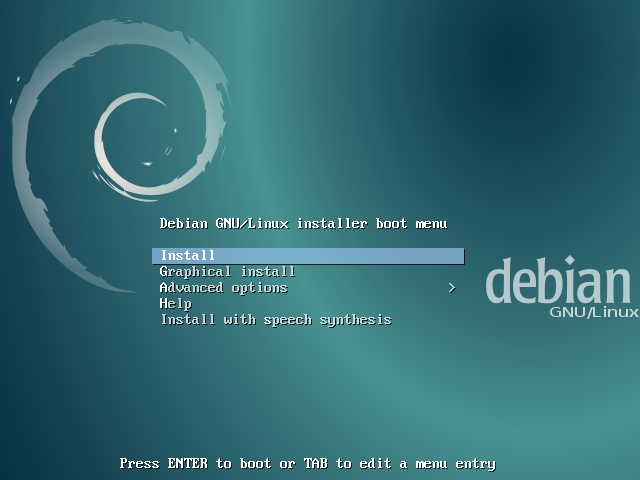
\includegraphics[width=0.8\hsize]{image201509/debian8-inst-01.png}
\caption{インストーラ起動直後}
\end{minipage}
\begin{minipage}{0.5\hsize}
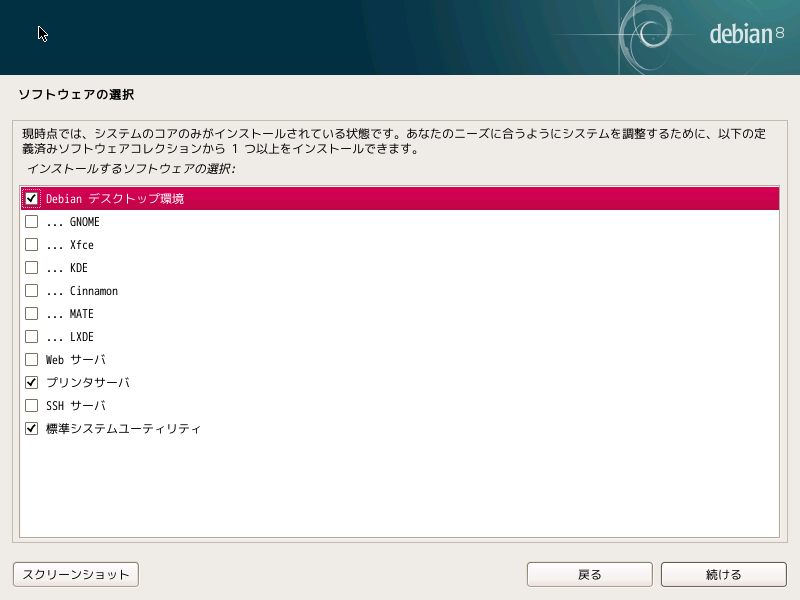
\includegraphics[width=0.8\hsize]{image201509/debian8-inst-02.png}
\caption{グラフィカルインストール}
\end{minipage}
\end{tabular}
\end{figure}

\end{frame}

\begin{frame}{ちょっとだけJessieおさらい(その4)}

\begin{figure}[htbp]
\begin{tabular}{cc}
\begin{minipage}{0.5\hsize}
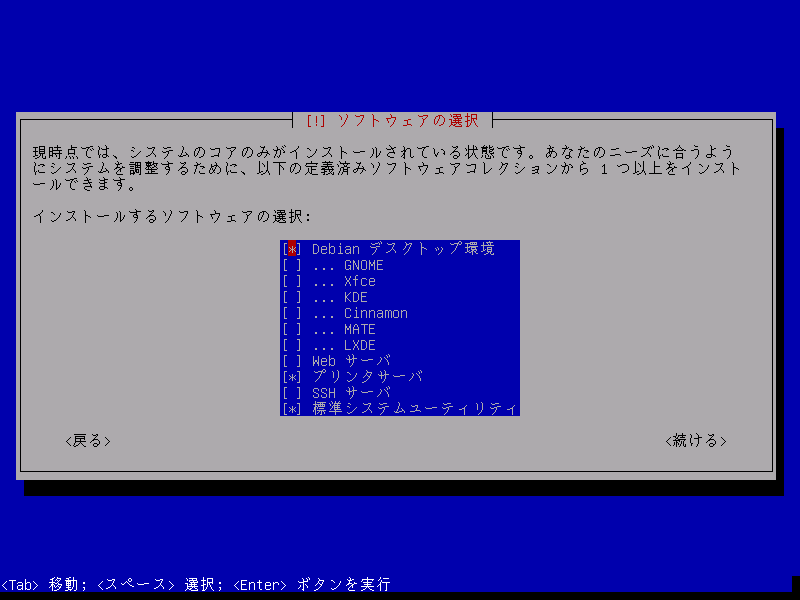
\includegraphics[width=0.8\hsize]{image201509/debian8-inst-03.png}
\caption{テキストインストール}
\end{minipage}
\begin{minipage}{0.5\hsize}
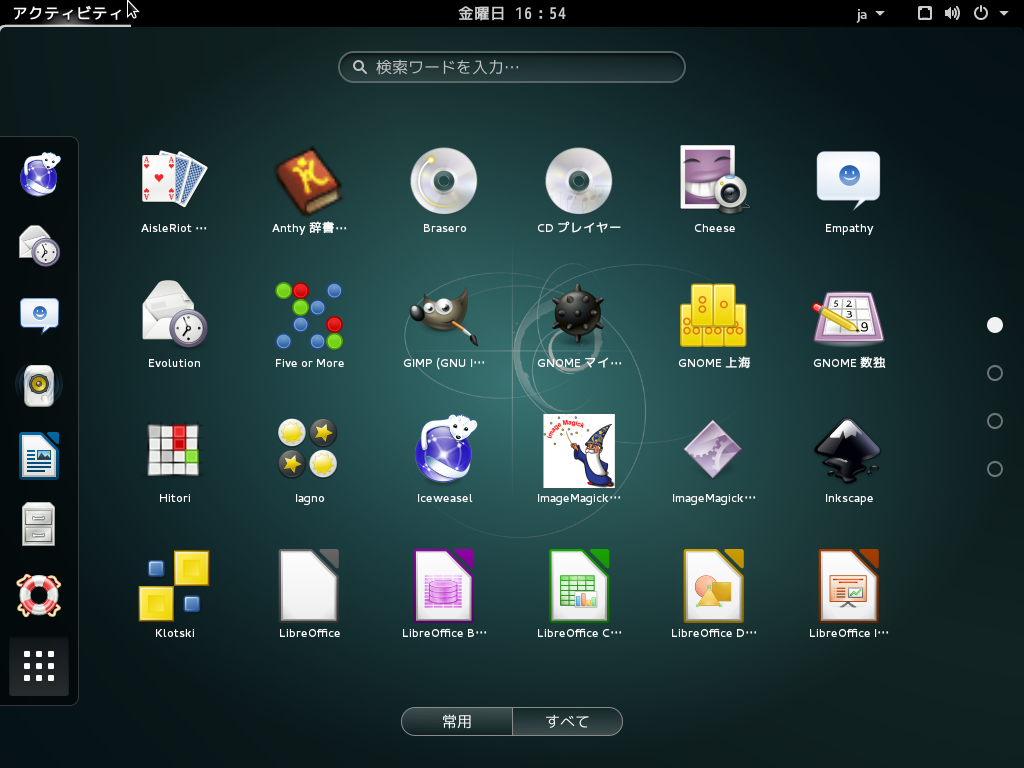
\includegraphics[width=0.8\hsize]{image201509/debian8-gnome.png}
\caption{GNOME環境}
\end{minipage}
\end{tabular}
\end{figure}

\end{frame}


\begin{frame}{ちょっとだけJessieおさらい(その5)}

\begin{figure}[htbp]
\begin{tabular}{cc}
\begin{minipage}{0.5\hsize}
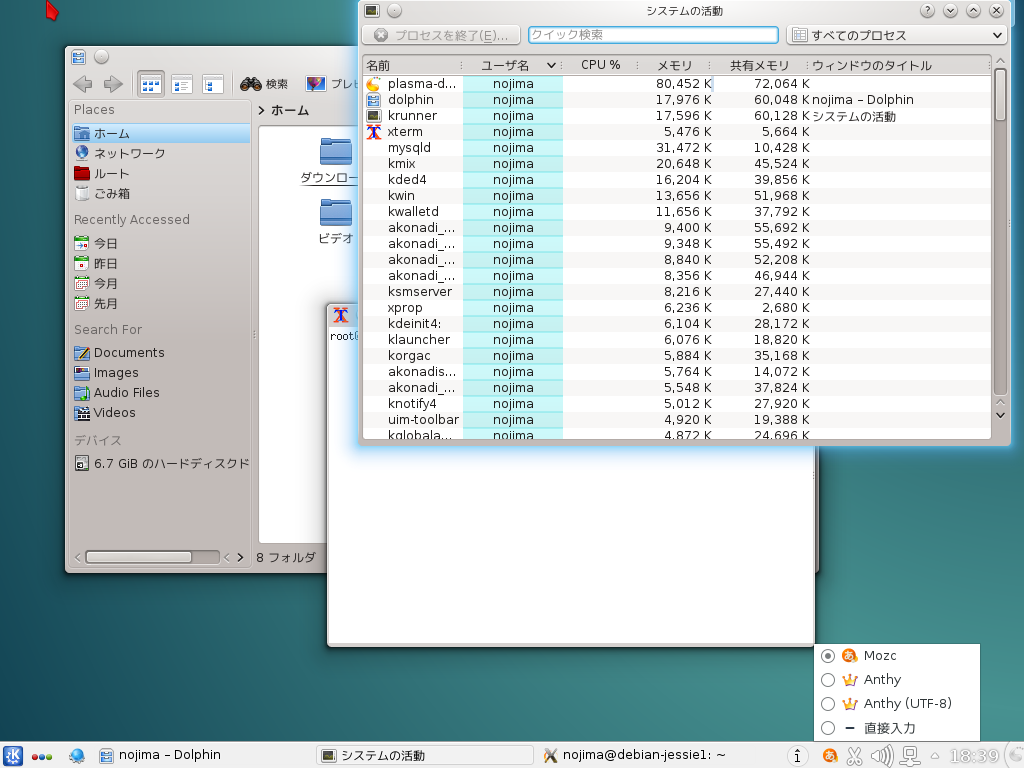
\includegraphics[width=0.8\hsize]{image201509/debian8-kde.png}
\caption{KDE環境}
\end{minipage}
\begin{minipage}{0.5\hsize}
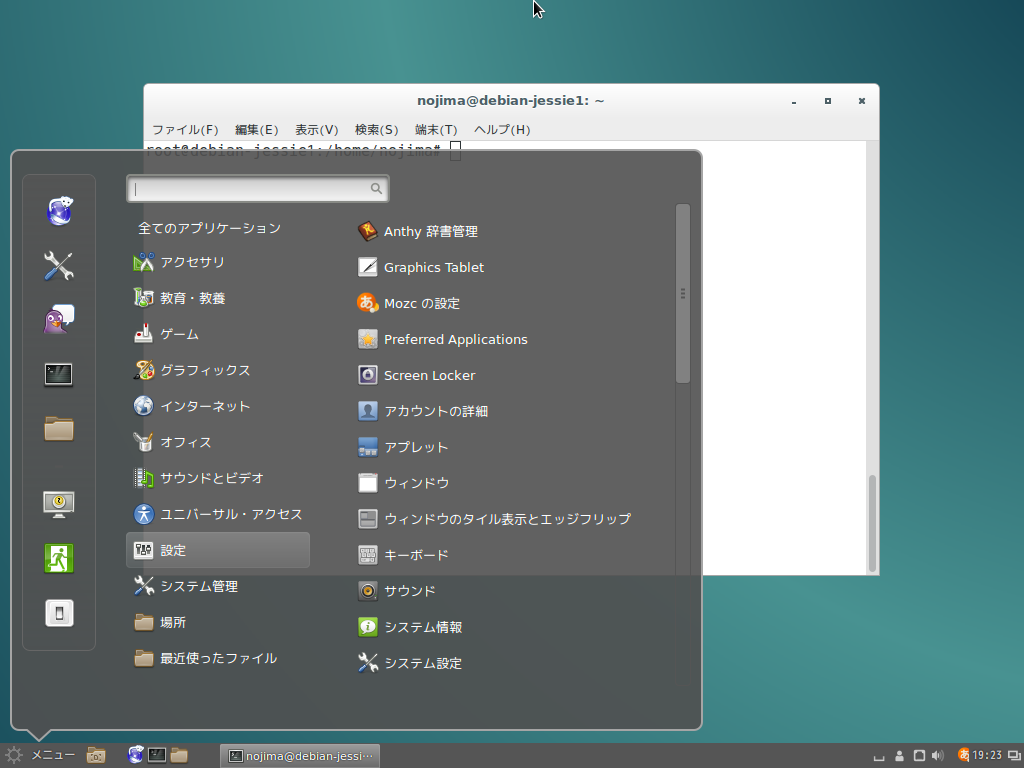
\includegraphics[width=0.8\hsize]{image201509/debian8-cinnamon.png}
\caption{cinnamon環境}
\end{minipage}
\end{tabular}
\end{figure}

\end{frame}

\begin{frame}{リリースその他}
  \begin{center}
    \Large
2015年4月30日 Debian GNU/Hurd 2015リリース
  \end{center}

\begin{itemize}
\item GNU Hurd 0.6ベース
\item GNU Mach 1.5搭載
\item とりあえずの動作なら、仮想環境で試せます。是非お試しあれ。
\end{itemize}

\end{frame}

\begin{frame}[containsverbatim]{Debian GNU/Hurd 2015 Live}

  Liveイメージもあるよ!\\
\url{https://www.gnu.org/software/hurd/hurd/running/debian.html}から抜粋

\begin{commandlinesmall}
# wget http://people.debian.org/~sthibault/hurd-i386/debian-hurd.img.tar.gz
# tar xz < debian-hurd.img.tar.gz
# kvm -m 512 -drive cache=writeback,file=debian-hurd-20150320.img
\end{commandlinesmall}
  
\end{frame}

\begin{frame}{Debian GNU/Hurd 2015 Live}

Debian GNU/Hurd 2015 Liveの様子。

\begin{center}
 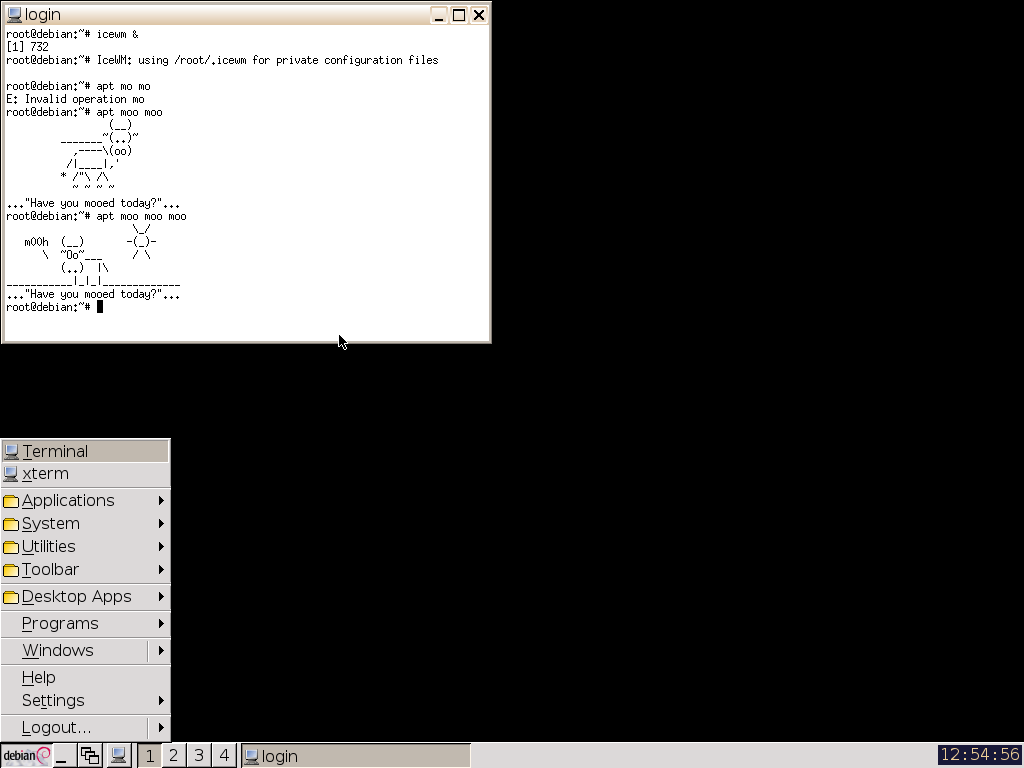
\includegraphics[width=0.9\hsize]{image201509/gnu-hurd-live.png}
\end{center}
 
\end{frame}

\emtext{その他}

\begin{frame}{次期バージョンのコード名}

  \begin{itemize}
  \item Debian 9 Stretch ←次回リリース
  \item Debian 10 Buster ←次々回リリース
  \end{itemize}
  
\end{frame}

\begin{frame}{Stretchスケジュール(予定)}

以下はStrechの開発に関する予定:

\begin{itemize}
  \item 2016年9月5日 Transition Freeze
  \item 2016年11月5日 Soft Freeze
  \item 2016年12月5日 Freeze
\end{itemize}

参照 DebConf15のリリースチームの動画:
http://caesar.acc.umu.se/pub/debian-meetings/2015/\\
debconf15/Onwards\_to\_Stretch\_and\_other\_items\\
\_from\_the\_Release\_Team.webm

\end{frame}

\begin{frame}{Stretchスケジュール(予定)}

 なお、Freezeはリリースの事ではないので注意。Strechに搭載する新規のパッケージの受付を完全にやめ、RCバグ潰しに専念しますという意味。
  
\end{frame}

\begin{frame}{gcc-5/libc++6 移行作業中}

 現在、開発版(sid)では、Stretchにて新しいバージョンのコンパイラでパッケージを構築できるようにするため、一旦gcc-5系列及び、libc++6の元でバイナリビルドできるようにする大作業が行われています。

\begin{itemize} 
\item ABIレベルで変更
\item C++11対応
\item GFortranでコンパイルするパッケージもこちの影響を受ける
\end{itemize}

\end{frame}

\begin{frame}{httpredir.debian.org稼働開始}

 ネットワーク観点から、もっとも近いdebianのmirrorサイトを紹介するサービスであった、
\begin{itemize}
  \item cdn.debian.net ... DNSクエリで、もっとも近いmirrorサイトを返す
  \item http.debian.net ... http redirectを使って、もっとも近いmirrorサイトを返す
\end{itemize}
が終了し、代わりのサービスとして、正式に httpredir.debian.orgが稼働しました。

\end{frame}

\begin{frame}[containsverbatim]{が、しかしhttpredir.debian.org}

  本来、
  \begin{commandlinesmall}
# cat /etc/apt/souces.list
deb http://httpredir.debian.org/debian/ jessie main
deb-src http://httpredir.debian.org/debian/ jessie main
deb http://httpredir.debian.org/debian/ jessie-updates main
deb-src http://httpredir.debian.org/debian/ jessie-updates main
#
  \end{commandlinesmall}
で、うまく近いmirrorが紹介されるはずが、何故か日本は精度が悪い状況です。インストーラによって設定されるftp.jp.debian.orgの方が現在は良いです。
    
\end{frame}

\begin{frame}{おしらせ}
\begin{itemize}
\item ブース出展中
\begin{itemize}
\item Debian マシン展示(Debian unstable搭載)
\item Debianキートップシール配布
\item 東京エリアDebian勉強会資料展示
\end{itemize}
\end{itemize}

\end{frame}

\begin{frame}{おしらせ(つづき)}
\begin{itemize}
\item イベント開催予定
\begin{itemize}
\item 東京エリアDebian勉強会(毎月開催)\\
  \url{http://tokyodebian.alioth.debian.org/}\\
  9月12日にパッケージ道場開催\\
  http://eventdots.jp/event/568568
\item 関西エリアDebian勉強会(毎月開催)\\
  \url{https://wiki.debian.org/KansaiDebianMeeting}
\item 各地OSC出展など。
\end{itemize}  
\end{itemize}
\end{frame}

\begin{frame}{質問}

\begin{center}
なにか質問はありますか?
\end{center}

\end{frame}


\end{document}

;;; Local Variables: ***
;;; outline-regexp: "\\([ 	]*\\\\\\(documentstyle\\|documentclass\\|emtext\\|section\\|begin{frame}\\)\\*?[ 	]*[[{]\\|[]+\\)" ***
;;; End: ***



%------

